\documentclass[12pt]{article}

\usepackage[brazilian]{babel}
\usepackage[utf8]{inputenc}
\usepackage{graphicx}
\usepackage{mathtools}
\usepackage{amsthm}
\usepackage{amssymb}
\usepackage{thmtools,thm-restate}
\usepackage{amsfonts}
\usepackage{hyperref}
\usepackage[singlelinecheck=false]{caption}
\usepackage[backend=biber,url=true,doi=true,eprint=false,style=numeric]{biblatex}
\usepackage{enumitem}
\usepackage[justification=centering]{caption}
\usepackage{indentfirst}
\usepackage{algorithm}
\usepackage[noend]{algpseudocode}
\usepackage{listings}
\usepackage[x11names,rgb,table]{xcolor}
\usepackage{tikz}
\usepackage{hyperref}
\usepackage{subcaption}
\usepackage{booktabs}
\usepackage{linegoal}
\usepackage{geometry}
\usetikzlibrary{snakes,arrows,shapes}

\addbibresource{references.bib}
\graphicspath{{imgs/}}

\makeatletter
\def\subsection{\@startsection{subsection}{3}%
  \z@{.5\linespacing\@plus.7\linespacing}{.1\linespacing}%
  {\normalfont}}
\makeatother

\makeatletter
\patchcmd{\@setauthors}{\MakeUppercase}{}{}{}
\makeatother

\DeclareMathOperator*{\argmin}{arg\,min}
\DeclareMathOperator*{\argmax}{arg\,max}
\DeclareMathOperator*{\Val}{\text{Val}}
\DeclareMathOperator*{\Ch}{\text{Ch}}
\DeclareMathOperator*{\Pa}{\text{Pa}}
\DeclareMathOperator*{\Sc}{\text{Sc}}
\newcommand{\ov}{\overline}
\newcommand{\tsup}{\textsuperscript}

\newcommand\defeq{\mathrel{\overset{\makebox[0pt]{\mbox{\normalfont\tiny\sffamily def}}}{=}}}

\newcommand{\algorithmautorefname}{Algorithm}
\algrenewcommand\algorithmicrequire{\textbf{Entrada}}
\algrenewcommand\algorithmicensure{\textbf{Saída}}
\algrenewcommand\algorithmicif{\textbf{se}}
\algrenewcommand\algorithmicthen{\textbf{então}}
\algrenewcommand\algorithmicelse{\textbf{senão}}
\algrenewcommand\algorithmicfor{\textbf{para todo}}
\algrenewcommand\algorithmicdo{\textbf{faça}}
\algnewcommand{\LineComment}[1]{\State\,\(\triangleright\) #1}

\captionsetup[table]{labelsep=space}

\theoremstyle{plain}

\newcounter{dummy-def}\numberwithin{dummy-def}{section}
\newtheorem{definition}[dummy-def]{Definition}
\newcounter{dummy-thm}\numberwithin{dummy-thm}{section}
\newtheorem{theorem}[dummy-thm]{Theorem}
\newcounter{dummy-prop}\numberwithin{dummy-prop}{section}
\newtheorem{proposition}[dummy-prop]{Proposition}
\newcounter{dummy-corollary}\numberwithin{dummy-corollary}{section}
\newtheorem{corollary}[dummy-corollary]{Corollary}
\newcounter{dummy-lemma}\numberwithin{dummy-lemma}{section}
\newtheorem{lemma}[dummy-lemma]{Lemma}
\newcounter{dummy-ex}\numberwithin{dummy-ex}{section}
\newtheorem{exercise}[dummy-ex]{Exercise}
\newcounter{dummy-eg}\numberwithin{dummy-eg}{section}
\newtheorem{example}[dummy-eg]{Example}

\numberwithin{equation}{section}

\newcommand{\set}[1]{\mathbf{#1}}
\newcommand{\pr}{\text{P}}
\newcommand{\eps}{\varepsilon}
\newcommand{\ddspn}[2]{\frac{\partial#1}{\partial#2}}
\newcommand{\iddspn}[2]{\partial#1/\partial#2}
\newcommand{\indep}{\perp}
\renewcommand{\implies}{\Rightarrow}

\newcommand{\bigo}{\mathcal{O}}

\setlength{\parskip}{1em}

\lstset{frameround=fttt,
	numbers=left,
	breaklines=true,
	keywordstyle=\bfseries,
	basicstyle=\ttfamily,
}

\newcommand{\code}[1]{\lstinline[mathescape=true]{#1}}
\newcommand{\mcode}[1]{\lstinline[mathescape]!#1!}

\title{%
  B-Splines\\~\\
  {\normalfont EP2 de MAC0210}
}
\author{Renato Lui Geh, NUSP: 8536030}
\date{}

\begin{document}

\maketitle

\section{Introdução}

O EP foi feito na linguagem Python. Foi usada a biblioteca pyglet\footnote{Disponível em
\url{https://bitbucket.org/pyglet/pyglet/wiki/Home}}, que age como um \textit{wrapper} de OpenGL
para Python. Toda a parte de desenho e GUI foi feita com esta biblioteca.

Para rodar o EP, é preciso do Python 3 e que a biblioteca pyglet esteja instalada. Além disso,
alguns cálculos foram feitos com NumPy. Foram usadas várias funções elaboradas durante o EP1.

\section{Uso}

O EP2, ao contrário do EP1, não é interativo. Ao invés disso, o usuário deve executar o EP2 da
seguinte forma.
\begin{lstlisting}[numbers=none]
$ python3 main.py
---
Usage: main.py data l
  data - dataset file
  l    - lambda constant for L2
\end{lstlisting}

Os parâmetros \code{data} e \code{l} são obrigatórios. O primeiro é o caminho para o arquivo de
dataset. O segundo é a constant $\lambda$ para regularização L2. O arquivo \code{data} é um
\code{plaintext} simples com o valor de cada par de valores $(t_i,y_i)$.  Abaixo segue um exemplo
de cinco pares deste formato.

\begin{lstlisting}[numbers=none]
$ cat in.put
---
0.000000000000000000e+00 4.229733993338091835e+01
1.000000000000000000e+00 4.242230348764690717e+01
2.000000000000000000e+00 4.093792562561398540e+01
3.000000000000000000e+00 4.009299524534277737e+01
4.000000000000000000e+00 4.108056259456515846e+01
...
\end{lstlisting}

Este arquivo é gerado através de um gerador aleatório \code{generator.py}. Para gerar um arquivo
\code{data}, requerem-se quatro parâmetros.

\begin{lstlisting}[numbers=none]
$ python3 generator.py
---
Usage: generator.py filename sdv n m
  filename - file name to save to
  sdv      - gaussian standard deviation to sample with
  n        - number of samples to generate
  m        - max value for samples
\end{lstlisting}

O primeiro, \code{filename}, refere-se ao nome do novo dataset file. O argumento \code{sdv} é o
valor do desvio padrão da gaussiana usada; \code{n} é o número de amostras a serem geradas; e
\code{m} é o valor máximo que cada valor $y_i$ pode alcançar.

A construção dos pares $(t_i,y_i)$ é bem simples, e é descrita no algoritmo abaixo.

\begin{algorithm}[h]
  \caption*{\textbf{Algoritmo 1.} \code{generator.py}: gerador de dataset}
  \begin{algorithmic}[1]
    \Require Desvio padrão $\sigma$, número de amostras $n$ e valor máximo $m$
    \Ensure Conjunto de pares $G$
    \State Seja $G$ uma lista vazia
    \State $\mu\gets \frac{m}{2}$
    \For{inteiro $i$ no intervalo $[0,n)$}
      \State Seja $\mu$ uma mostra de $\mathcal{N}(\mu,\sigma^2)$
      \If{$\mu>m$}
        \State $mu\gets mu - 2\sigma$
      \ElsIf{$\mu<0$}%
        \State $mu\gets mu + 2\sigma$
      \EndIf
      \State Insere par $(i, \mu)$ em $G$
    \EndFor%
    \State\textbf{retorna} $G$
  \end{algorithmic}
\end{algorithm}

Desta forma garante-se que todos valores estejam no intervalo $[0, m]$. Como são amostrados por uma
gaussiana, podemos amostrar diferentes curvas alterando o valor de $\sigma$. Quanto maior $\sigma$,
mais ``bruscas'' as curvas.

Abaixo segue um exemplo de escolha de parâmetros.

\begin{lstlisting}[numbers=none]
$ python3 generator.py in.put 2 200 40
\end{lstlisting}

Depois de gerado o dataset, podemos desenhar a spline.

\begin{lstlisting}[numbers=none]
$ python3 main.py in.put 0.01
\end{lstlisting}

Este comando desenhará uma spline com um $\lambda=0.01$ para regularização L2. A~\autoref{fig:1} é
um exemplo de uma spline desenhada a partir dos pares de pontos gerados pelo gerador. Os pontos em
vermelho mostram os pontos reais do dataset. A curva em azul mostra os valores da spline

\begin{equation*}
  S(t)=\sum_{i=0}^n a_i\beta(t-i)
\end{equation*}

para cada valor em $[0,n)$, onde $\beta$ é a spline básica usada e $a$ é o vetor de coeficientes.

Alterando o $\lambda$ e o número de splines usadas é possível observar como a curva muda. De fato,
é possível perceber que a curva sofre ``overfitting'' quando $\lambda$ tende a zero.
A~\autoref{fig:2} mostra este fenômeno sem mudar o número de splines básicas usadas.
\begin{figure}[h]
  \centering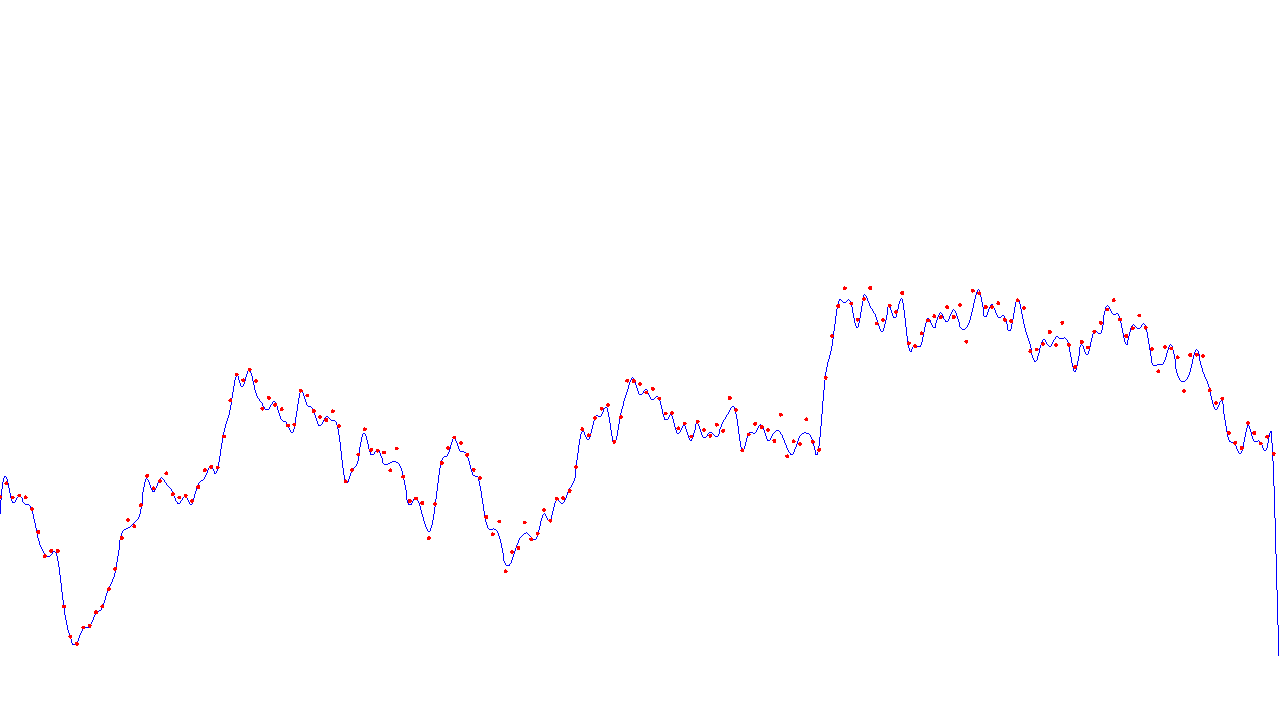
\includegraphics[width=0.925\textwidth]{imgs/200_0-01.png}
  \caption{Spline desenhada com $\lambda=0.01$ e 200 amostras.\label{fig:1}}
\end{figure}
\begin{figure}[H]
  \centering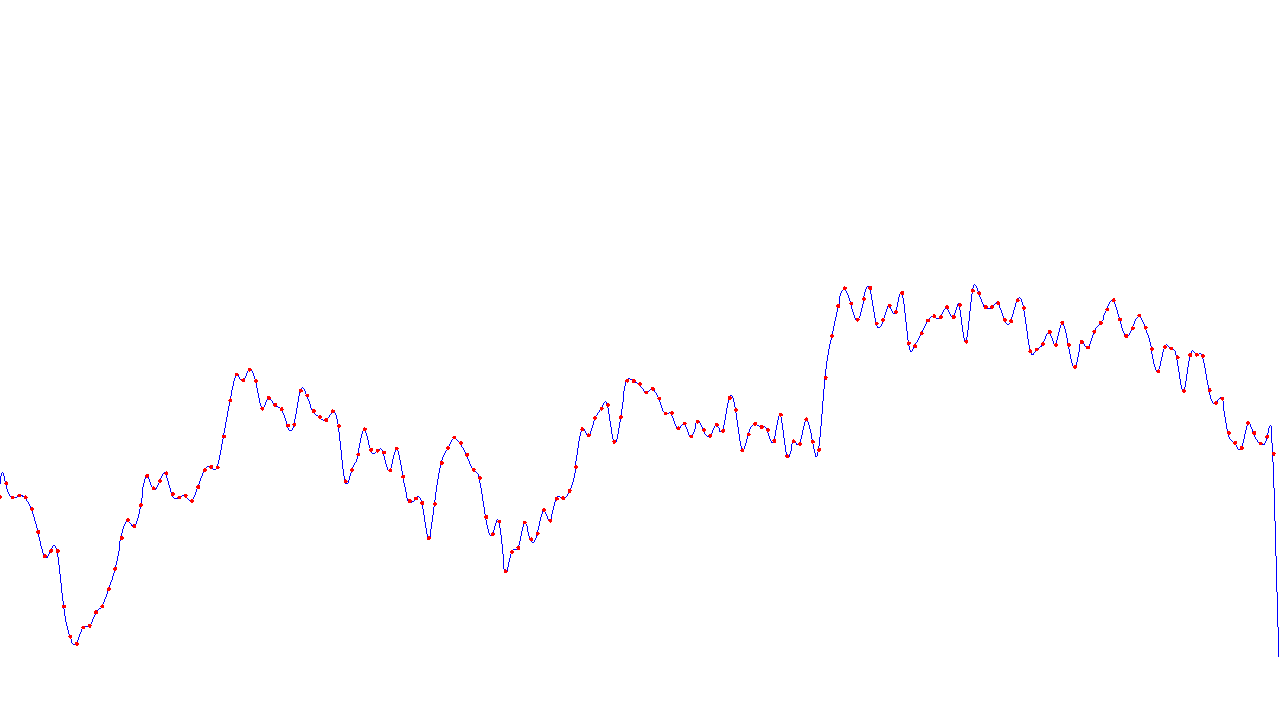
\includegraphics[width=0.925\textwidth]{imgs/200_0-0001.png}
  \caption{Spline desenhada com $\lambda=0.0001$ e 200 amostras.\label{fig:2}}
\end{figure}

Quando $\lambda$ é muito grande (no caso observei empíricamente que isso ocorre quando
$\lambda\geq0.1$), a curva perde o sentido, aumentando o erro demais, como mostra
a~\autoref{fig:2}.
\vspace{-1cm}
\begin{figure}[h]
  \centering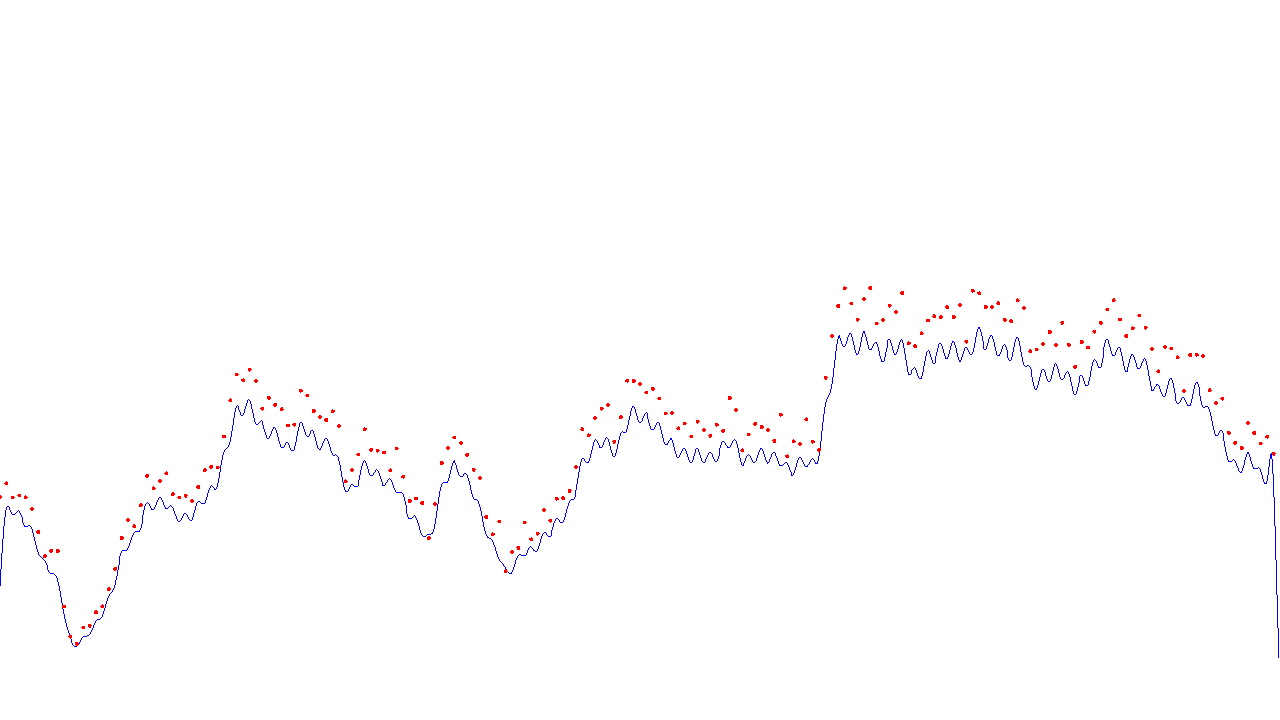
\includegraphics[width=0.9\textwidth]{imgs/200_0-1.png}
  \caption{Spline desenhada com $\lambda=0.1$ e 200 amostras.\label{fig:3}}
\end{figure}

Com poucas amostras podemos observar melhor a suavidade da curva com um $\lambda$ maior.
\vspace{-1cm}
\begin{figure}[H]
  \centering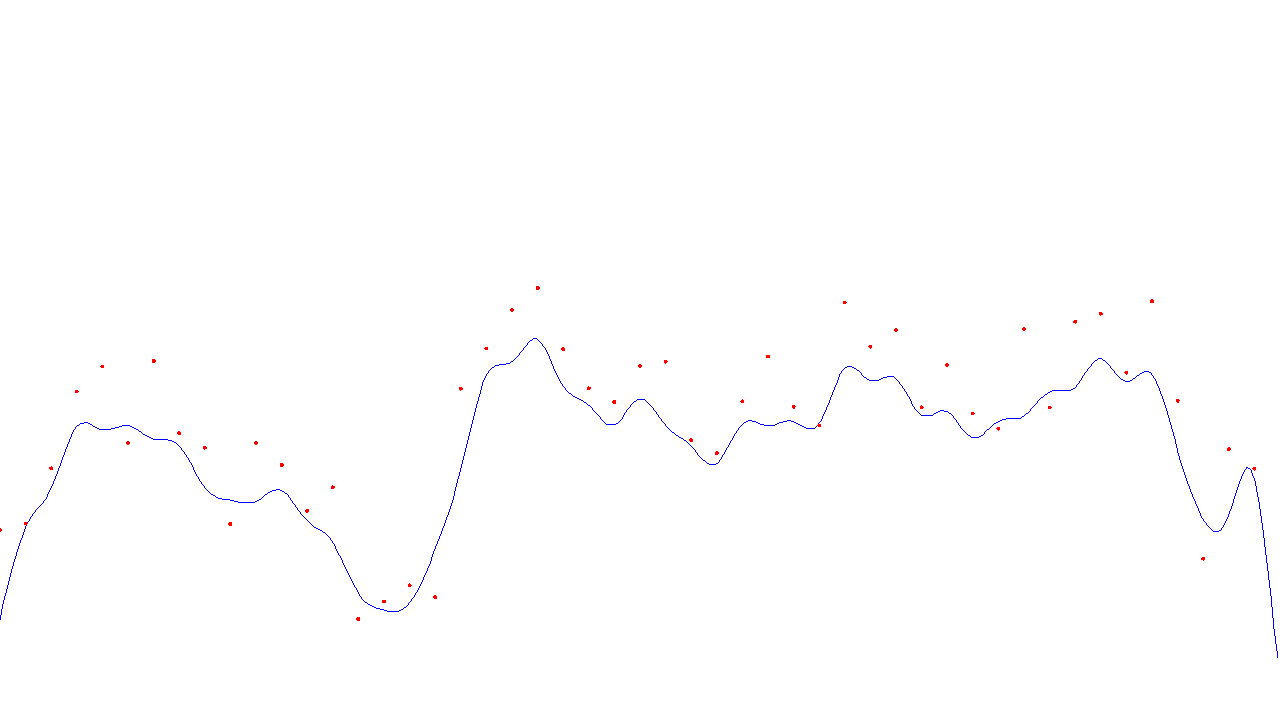
\includegraphics[width=0.9\textwidth]{imgs/50_0-1.png}
  \caption{Spline desenhada com $\lambda=0.1$ e 50 amostras.\label{fig:5}}
\end{figure}

\begin{figure}[h]
  \centering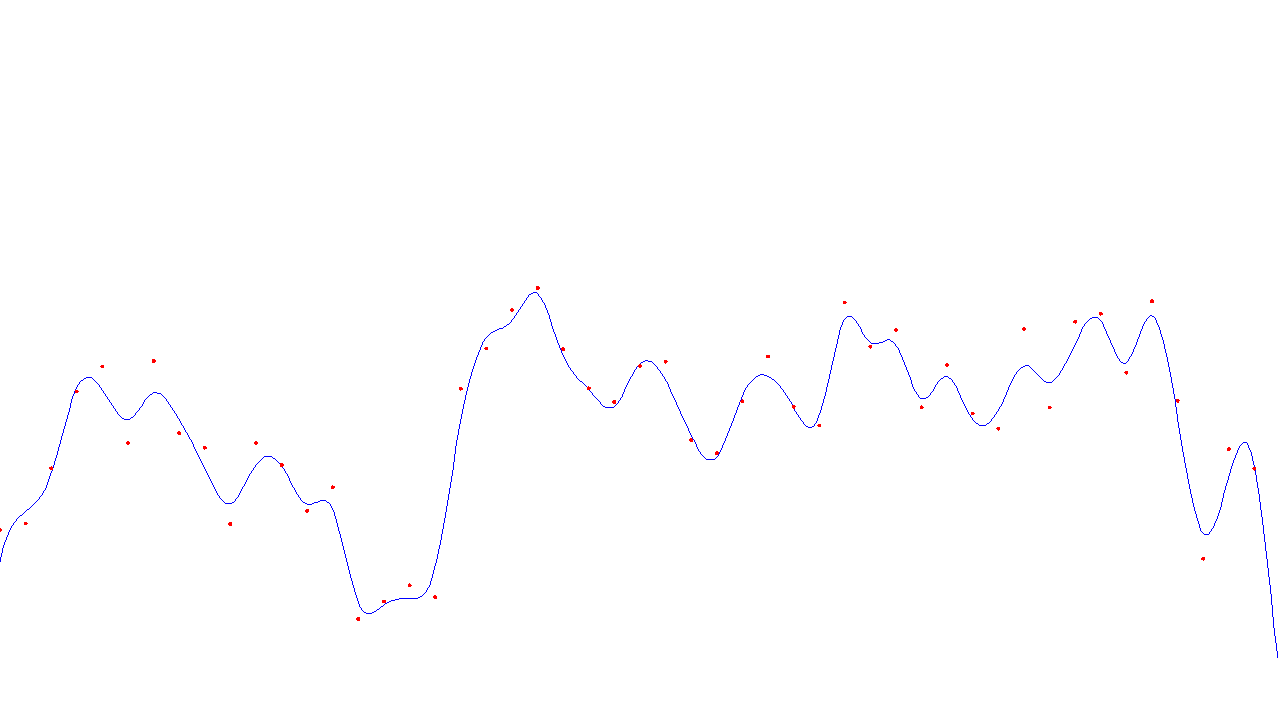
\includegraphics[width=1.0\textwidth]{imgs/50_0-01.png}
  \caption{Spline desenhada com $\lambda=0.01$ e 50 amostras.\label{fig:4}}
\end{figure}

\begin{figure}[H]
  \centering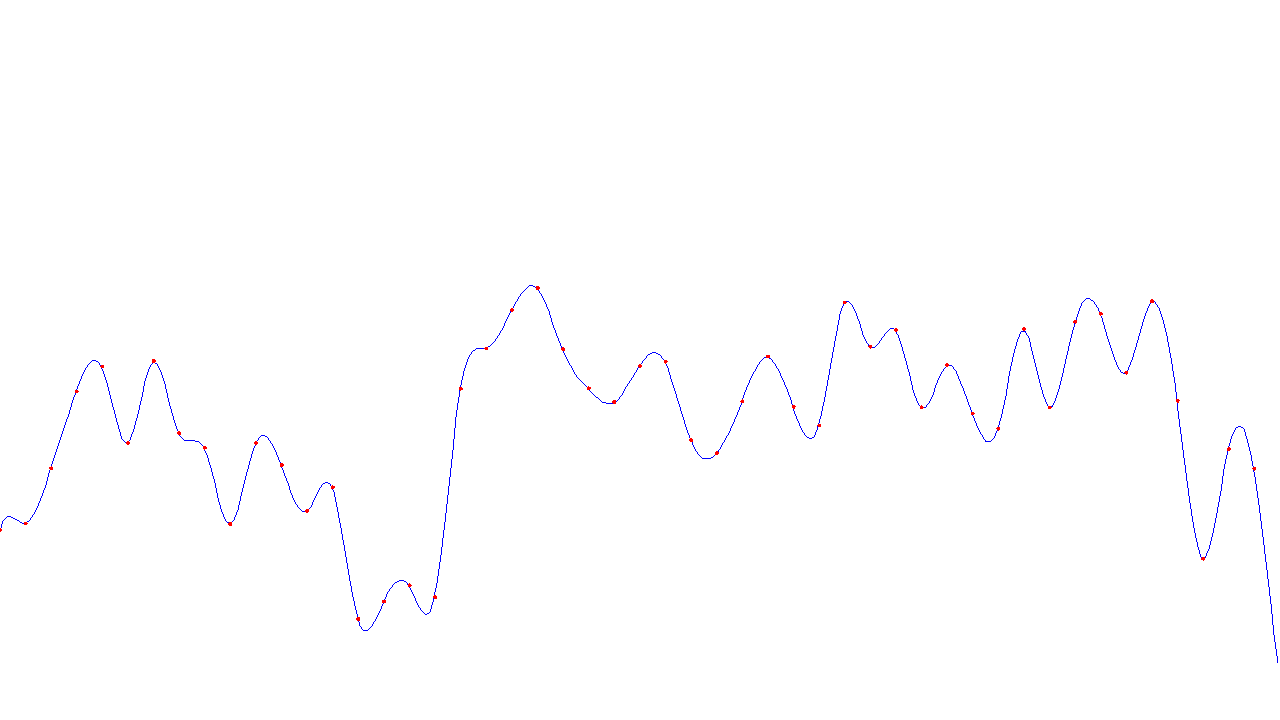
\includegraphics[width=1.0\textwidth]{imgs/50_0-0001.png}
  \caption{Spline desenhada com $\lambda=0.0001$ e 50 amostras.\label{fig:5}}
\end{figure}

\section{Estrutura do código}

Em \code{main.py}, lêem-se os parâmetros dados pela \code{command line} e em seguida cria-se uma
instância da classe \code{Dataset}, que agrupa os pares $(t_i,y_i)$ para serem lidos pela spline.
Após a criação do \code{Dataset}, é gerada a janela e a tela de desenho.

O arquivo \code{frame.py} define a janela e cuida de desenhar os elementos no canvas do OpenGL.
A classe \code{Frame}, que representa a janela e o canvas, cria a classe \code{Spline} e passa o
\code{Dataset} a ela.

Para construir a spline, computa-se primeira a matriz $M$ definida por

\begin{equation*}
  M_{i,j}=2\int_0^n \beta(t-i)\beta(t-j)\mathrm{d}t,
\end{equation*}

onde $n$ define um bound para $t_i$ tal que $0\leq t_i\leq n$. Esta matriz independe do conjunto de
dados, e portanto é pré-computada.

Em seguida, usa-se o método \code{Spline.fit(data, lambda)} para achar um vetor de coeficientes
$a\in\mathbb{R}^n$ que modelem o conjunto de dados \code{data} com constante de regularização L2
$\lambda=$ \code{lambda}. Para isso, constrói-se a matriz $B$ onde cada elemento toma a forma

\begin{equation*}
  B_{i,j}=\beta(t_i-j).
\end{equation*}

A matriz $M$ é esparsa, já que quando $|t-k|>2$, $\beta(t-k)=0$. Portanto, podemos evitar computar
os valores de cada elemento de $M$, que demoraria tempo $\bigo(n^2)$, e ao invés disso computar
apenas a região da diagonal até uma distância dois para cada lado. Deste jeito, é possível computar
$M$ em tempo $\bigo(n)$.

O algoritmo abaixo computa $M$ em tempo linear. Para computar o valor da integral abaixo, usa-se a
lei de Simpson, que simplifiquei para o intervalo $[0,n]$:

\begin{equation*}
  \int_{0}^n f(x)\mathrm{d}x\approx f(0)+f(n)+\sum_{i=1}^n 2^{(i\mod 2)+1}f(i)
\end{equation*}

\begin{algorithm}[h]
  \caption*{\textbf{Algoritmo 2.} \code{Computa} $M$}
  \begin{algorithmic}[1]
    \Require Bound $n$ tal que $0\leq t_i\leq n$ é válido para todo $t_i\in D$, $D$ dataset
    \Ensure Matriz $M$
    \State Seja $M$ uma matriz nula de dimensão $n\times n$
    \For{inteiro $i$ no intervalo $[0,n)$}
      \For{inteiro $d$ no intervalo $[-4, 4]$}
        \State $j\gets i+d$
        \If{$j\geq 0$ e $j<n$}
          \State $M_{i,j}\gets 2\int_0^n \beta(t-i)\beta(t-j)\mathrm{d}t$
        \EndIf%
      \EndFor%
    \EndFor%
    \State\textbf{retorna} $M$
  \end{algorithmic}
\end{algorithm}

A matriz $B$ é um tanto diferente, e o mesmo raciocínio não pode ser aplicado neste caso. Já que
$B$ depende de cada valor $t_i$ do conjunto de dados, não basta apenas computar a diagonal, já que
o conjunto pode não estar ordenado. Portanto, acabei deixando $\bigo(nm)$. Como assume-se que $n$ é
relativamente pequeno, podemos considerar isso praticamente linear.

Agora que temos $B$ e $M$, podemos computar o vetor coeficiente a partir da derivação do gradiente.

\begin{equation*}
  \nabla f(a)=(B^\intercal B+\lambda M)a-B^\intercal y=0\implies (B^\intercal B+\lambda
  M)a=B^\intercal y
\end{equation*}

\begin{algorithm}[h]
  \caption*{\textbf{Algoritmo 3.} \code{Computa} $a$}
  \begin{algorithmic}[1]
    \Require Matrizes $M$ e $B$, vetor $y$ do dataset e constante $\lambda$
    \Ensure Vetor de coeficientes $a$
    \State $A\gets B^\intercal B+\lambda M$
    \State $b\gets B^\intercal y$
    \State Soluciona sistema linear $Ax=b$ em função de $x$
    \State $a\gets x$
    \State\textbf{retorna} $a$
  \end{algorithmic}
\end{algorithm}

Para achar a solução do sistema linear, usou-se \code{numpy.linalg.solve}.

Agora que temos $a$, podemos desenhar a spline. Para isso, decidi percorrer por ``todo'' (tomando
um certo $\epsilon$ suficientemente pequeno para a iteração) o domínio da spline $S$, e para valor
de $t$ no domínio, achar o valor de

\begin{equation}
  S(t)=\sum_{i=0}^n a_i\beta(t-i).\label{eq:1}
\end{equation}

No entanto, esta tarefa é $\bigo(nm)$, e será computada para cada instante de renderização.
Portanto precisei otimizar esta parte do código. Otimizar esta soma foi fácil. É fácil ver que
$\beta(t-i)=0$ no intervalo $[-4,4]$. Neste caso, podemos substituir a~\autoref{eq:1} pela forma

\begin{equation*}
  S(t)=\sum_{i=t-2}^{t+2} a_i\beta(t-i).
\end{equation*}

O algoritmo fica portanto:

\begin{algorithm}[h]
  \caption*{\textbf{Algoritmo 4.} \code{Computa} $S(t)$}
  \begin{algorithmic}[1]
    \Require $t\in\mathbb{R}$
    \Ensure $S(t)$
    \State $z\gets 0$
    \For{inteiro $i$ no intervalo $[-4,4]$}
      \State $k\gets\lfloor t\rfloor+i$
      \If{$k\geq 0$ e $k<n$}
        \State $z\gets z+a_k\beta(t-k)$
      \EndIf%
    \EndFor%
    \State\textbf{retorna} $z$
  \end{algorithmic}
\end{algorithm}

A função $\beta$ escolhida foi:

\begin{align*}
  \beta(t)=\begin{cases}
    \frac{(2-t)^3}{4} & \quad \text{, se }1\leq t<2;\\
    \frac{3t^3}{4}-\frac{3t^2}{2}+1 & \quad \text{, se }0\leq t<1;\\
    \frac{-3t^3}{4}-\frac{3t^2}{2}+1 & \quad \text{, se }-1\leq t<0;\\
    \frac{(t+2)^3}{4} & \quad \text{, caso contrário.}
  \end{cases}
\end{align*}

Por causa desta escolha, $\beta$ toma valores não zero apenas no domínio $[-4,4]$, e tem imagem em
apenas $[0,1]$. Isto trouxe problemas na hora de desenhar a spline, já que consideramos cada
unidade atômica um píxel. Para solucionar este problema, aplicamos uma escala durante a computação
de $S(t)$.

Desenhar cada valor de $S(t)$ consistia em desenhar o ponto $(s_x\cdot t, s_y\cdot S(t))$. Esta
escala foi escolhida a partir dos valores do tamanho da janela, e de $n$ e $m$. Seja $w$ e $h$ as
dimensões da janela.

\begin{align*}
  &s_x = w/n\\
  &s_y = 0.6\frac{h}{\max\{y^\ast\in y\}}
\end{align*}

Desta forma, toda a spline fica visível na tela, desde o primeiro ponto até o último. Além disso,
pela escala $s_y$, a spline fica mais ou menos no meio da tela.

\printbibliography[]

\end{document}
